\documentclass[tikz]{standalone}
\usepackage{tikz}
\usetikzlibrary{bayesnet}
\begin{document}
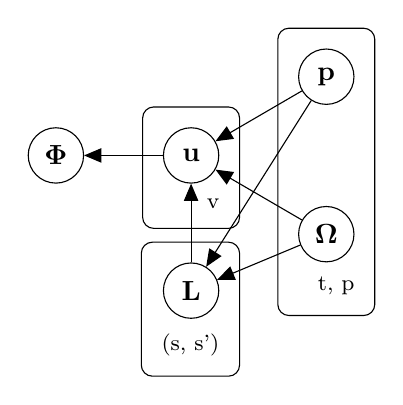
\begin{tikzpicture}

%Declare nodes.
\node[latent] (phi) {$\mathbf{\Phi}$};
\node[latent, right=of phi] (u) {$\mathbf{u}$};
\node[latent, below=of u] (L) {$\mathbf{L}$};
\node[latent, right=of u, yshift=-1cm] (omega) {$\mathbf{\Omega}$};
\node[latent, right=of u, yshift=1cm] (p) {$\mathbf{p}$};
		
%Setup plates.
\plate[inner sep=0.25cm] {plate1} {(omega) (p)} {t, p};
\plate[inner sep=0.25cm] {plate2} {(u)} {v};
\plate[inner sep=0.25cm] {plate3} {(L)} {(s, s')};
		
%Setup edges.
\edge {omega, p} {u, L}
\edge {L} {u}
\edge {u} {phi}

\end{tikzpicture}
\end{document}